%!TEX TS-program = xelatex

\documentclass[]{friggeri-cv}
\usepackage{ctex}
\usepackage{afterpage}
\usepackage{hyperref}
\usepackage{color}
\usepackage{xcolor}
\hypersetup{
    pdftitle={},
    pdfauthor={Feng},
    pdfsubject={},
    pdfkeywords={resume},
    colorlinks=false,       % no lik border color
   allbordercolors=white    % white border color for all
}
\addbibresource{bibliography.bib}
\RequirePackage{xcolor}
\definecolor{pblue}{HTML}{0395DE}
%header
\begin{document}
\header{厦门}{四三九九}
      { 彭峰 } 
      
 %对应cls中的  node的三个   

% Fake text to add separator      
\fcolorbox{white}{gray}{\parbox{\dimexpr\textwidth-2\fboxsep-2\fboxrule}{%
.....
}}


\begin{aside}
  \section{工作意向}
    系统运维工程师
    ~
  \section{Phone \& Skype}
    17091314725
    ms6577
    ~
  \section{Email}
    \href{mailto:git4xuan@gmail.com}{\textbf{git4xuan@}\\gmail.com}
    \href{mailto:jobs@fengidea.com}{\textbf{jobs@}\\fengidea.com}
    ~
%  \section{在线简历}
%    \href{http://devops.mxuan.me}{devops.mxuan.me}
%    \href{https://bitbucket.org/neoben}{bitbucket.org/neoben}
%    \href{https://github.com/neoben}{github.com/neoben}
    ~
  \section{Programming}
  ~
    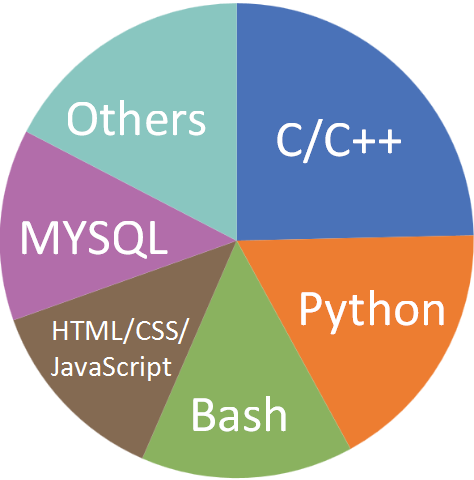
\includegraphics[scale=0.25]{img/programming2.png}
    ~
  \section{OS Preference}
  ~
    \textbf{openSUSE}
\includegraphics[scale=0.40]{img/5stars.png}
    \textbf{Debian}
\includegraphics[scale=0.40]{img/4stars.png}
    \textbf{CentOS}
\includegraphics[scale=0.40]{img/3stars.png}
    \textbf{Windows}
\includegraphics[scale=0.40]{img/3stars.png}
  ~
  \section{Tag}
  ~
  \textbf{TCP/IP}
\includegraphics[scale=0.40]{img/4stars.png}
  \textbf{Nginx}
\includegraphics[scale=0.40]{img/4stars.png}
  \textbf{Vim}
\includegraphics[scale=0.40]{img/3stars.png}
  \textbf{Docker}
\includegraphics[scale=0.40]{img/2stars.png}
  \textbf{Puppet}
\includegraphics[scale=0.40]{img/2stars.png}
  \textbf{Zabbix}
\includegraphics[scale=0.40]{img/2stars.png}
  \textbf{AWS}
\includegraphics[scale=0.40]{img/2stars.png}
  ~
\end{aside}

\section{项目介绍}
\begin{entrylist}
  \entry
    {02/15 - 05/15}
    {嵌入式显微成像系统}
    {Django}
    {在树莓派的基础上搭建的系统平台,在嵌入式系统下对光学薄膜进行数字显微成像和基本的图像处理,并可以远程显示和控制。内核进行系统配置实现集成化。硬件部分包括了光学衔接系统、显微采集硬件模块、光源设计等;Web界面实现图片显示与管理、基本图像处理等功能。整体使用B/S架构,Server端使用七牛API,并利用Docker进行部署。
   \\ }%考虑自己如何自己进行扩展,以及细节部分

   \entry
   {10/13 - 01/14}
   {基于树莓派的移动摄影车}
   {RaspberryPi}
   {
    树莓派在教育和ARM方面取得巨大的影响。项目中小车由Android客户端进行控制,Python调用GPIO接口利用L298N驱动板控制小车运动方向,使用USB接口的网络摄像头采集图像,在局域网下,以Web界面作为图像和视频的显示方式。个人负责任务协调,硬件设计和组装,以及Web界面。
   }
   
\end{entrylist}

\section{技能实践}
\begin{entrylist}
  \entry
    {02/15 - 08/15 }
    {虚拟化技术与平台}
    {Virtualization}
    {基于openSUSE 13.2的KVM。逻辑上简单参照Openstack,在硬盘上划分分区作为块分区的存储池,制作自用镜像。构建内网桥接环境和外网NAT环境。补充virt-manager中没有图形化实现的部分功能,编写CLI,在virsh和xml配置的基础上制定特定的虚拟机资源类型模板等,从而快速根据自身需要创建和使用干净的测试和学习环境。
    \\}   
	{
	
	
	}
  \entry
    {03/14 - 07/14 }
    {文件存储与共享}
    {Storage}
    {提供家庭一站式文件存储与共享功能,系统基于openSUSE,在局域网内利用KVM虚拟化提供SAMBA、NFS共享、FTP、DLNA、LEMP基础上搭建owncloud个人云等服务。\\}%注意要和用户权限控制联系 还有swift相关
    



\end{entrylist}

\section{校内经历}
\begin{entrylist}
  \entry
    {07/13 - 04/14}
    {校科协信息化实验室管理员}
    {系统与服务}
    {\emph{服务器搭建与技术支持}
    适逢实验室添加新设备,负责计算机和交换机上报选型,为校科协多个部门提供技术支持和服务。包括:使用WindowsServer2008 R2实现路由和远程桌面服务,提供局域网内公共FTP和部门FTP文件共享,提供常见软件的安装和使用,部分Adobe系列软件培训,解决基本的网络问题。较好的实现了第一年实验室的技术支撑。  \\     
    }
    
\end{entrylist}


\newpage


\begin{aside}
~
~
  \section{Languages}
    \textbf{English}
\includegraphics[scale=0.40]{img/4stars.png}
  ~    
    \section{Personal Skills}
    ~
    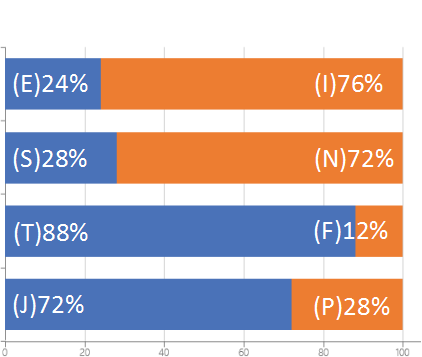
\includegraphics[scale=0.72]{img/personal.png}
    ~
\end{aside}




\section{教育背景}
08/12\hspace{1mm}-\hspace{1mm}至今 \hspace{30mm} 电子科学与技术 \hspace{7mm}  西安电子科技大学  \hspace{7mm}  本科 \\

相关课程与内容:数字电路,微机原理,电子元器件,光纤通信与应用,计算机图形学。\\


\section{其他信息}
To HR:\\
\emph{您好,我叫彭峰,西电本科生,这里应聘的是系统运维,我认为在运维部门中,更需要熟悉运维需求的同时,又能有一定开发能力的人。为此,简历主要展示的是Linux运维的能力和Web开发(Python)的能力。当然,基础的知识也是不可缺的。
我知道春招可能连名额都没有,所以,如果还有名额空缺的话,希望能给一次电面的机会。\\
%简历下载链接:\href{http://fengidea.qiniudn.com/系统运维工程师-西电-58-彭峰.pdf}{系统运维工程师-西电-58-彭峰.pdf}
最后,非常感谢您花时间来阅读这份简历!\\
}

{简历下载链接:\href{http://fengidea.qiniudn.com/系统运维工程师-西电-58-彭峰.pdf}{系统运维工程师-西电-58-彭峰.pdf}}
~
~
\begin{flushleft}
\emph{2/18/2016}
\end{flushleft}
\begin{flushright}
\emph{彭峰}
\end{flushright}


\end{document}
